\documentclass[sigconf]{acmart}

\usepackage{booktabs} % For formal tables

\usepackage{graphicx}

% Copyright
%\setcopyright{none}
%\setcopyright{acmcopyright}
%\setcopyright{acmlicensed}
\setcopyright{rightsretained}
%\setcopyright{usgov}
%\setcopyright{usgovmixed}
%\setcopyright{cagov}
%\setcopyright{cagovmixed}


% % DOI
% \acmDOI{10.475/123_4}
% 
% % ISBN
% \acmISBN{123-4567-24-567/08/06}
% 
% %Conference
% \acmConference[AVI2018]{ACM Woodstock conference}{July 2018}
%               {Rome, Italy}
% \acmYear{2018}
% \copyrightyear{2018}
% 
% 
% \acmArticle{4}
% \acmPrice{15.00}

% These commands are optional
%\acmBooktitle{Transactions of the ACM Woodstock conference}
% \editor{Jennifer B. Sartor}
% \editor{Theo D'Hondt}
% \editor{Wolfgang De Meuter}


\begin{document}
\title{EpisoDAS - DAS-based password generation \\
using episodic memories}
% \titlenote{Produces the permission block, and copyright information}

\author{Toshiyuki Masui}
% \authornote{Is this necessary?.}
\orcid{1234-5678-9012}
\affiliation{%
  \institution{Keio University}
  \streetaddress{Endo}
  \city{Fujisawa}
  \state{Kanagawa}
  \postcode{43017-6221}
}
\email{masui@masui.org}

\renewcommand{\shortauthors}{T. Masui}

\begin{abstract}

We introduce a simple and powerful visual interaction technique for
managing strong passwords.  Passwords have been used for
qauthentication for decades, but appropriate handling of passwords is
difficult because people can easily forget passwords and they can be
easily cracked.
%
To make the authentication process easier, various visual interaction
methods have been proposed, including the DAS (draw-a-secret)
method. Using DAS, users can log into various services just by drawing
a secret pattern on the screen.
%
Using a DAS-based authentication method, users can quickly log into a
service without typing a password. However, remembering complex secret
patterns can be as difficult as remembering passwords. We developed
EpisoDAS, with which users can generate strong passwords based on
their secret episodic memories with a simple DAS interface.
%
users can use secret patterns for authentication, based on their
secret episodic memories which they cannot easily forget.

\end{abstract}

%
% The code below should be generated by the tool at
% http://dl.acm.org/ccs.cfm
% Please copy and paste the code instead of the example below.
%
% \begin{CCSXML}
% <ccs2012>
%  <concept>
%   <concept_id>10010520.10010553.10010562</concept_id>
%   <concept_desc>Computer systems organization~Embedded systems</concept_desc>
%   <concept_significance>500</concept_significance>
%  </concept>
%  <concept>
%   <concept_id>10010520.10010575.10010755</concept_id>
%   <concept_desc>Computer systems organization~Redundancy</concept_desc>
%   <concept_significance>300</concept_significance>
%  </concept>
%  <concept>
%   <concept_id>10010520.10010553.10010554</concept_id>
%   <concept_desc>Computer systems organization~Robotics</concept_desc>
%   <concept_significance>100</concept_significance>
%  </concept>
%  <concept>
%   <concept_id>10003033.10003083.10003095</concept_id>
%   <concept_desc>Networks~Network reliability</concept_desc>
%   <concept_significance>100</concept_significance>
%  </concept>
% </ccs2012>
% \end{CCSXML}

% \ccsdesc[500]{Computer systems organization~Embedded systems}
% \ccsdesc[300]{Computer systems organization~Redundancy}
% \ccsdesc{Computer systems organization~Robotics}
% \ccsdesc[100]{Networks~Network reliability}


% \keywords{ACM proceedings, \LaTeX, text tagging}

\maketitle

%\input{samplebody-conf}
\section{Introduction}

Passwords have been used as a means of authenticating to Web services
and applications for a long time, and remain the most popular
authentication method on the Internet.
Since short passwords are easily guessable by attackers and using the
same password for multiple services is unsafe, a different long
password should be used for each service a person uses.  However,
remembering numerous long passwords is almost impossible for ordinary
humans.

However, password-based authentication is still the most convenient
and widely deployed method \cite{Bonneau:ReplacePasswords}, and is not
expected to disappear any time soon \cite{Herley:2009:PSS:1601990.1602010}.

We have been proposing the \textit{EpisoPass} password generator with which 
users can generate strong passwords easily
based only on a user's secret and unforgettable episodic memories.

% For this reason, we believe that it is far better to ``generate''
% something for the authentication, based on a user's episodic
% memories. This has the benefit that unlike a password, a person is
% highly unlikely to forget such episodic memories.

\begin{figure}
  \centerline{\includegraphics[width=9cm,bb=0 0 1522 1114]{figures/episopass.png}}
  \caption{EpisoPass}
  \label{fig:sample}
\end{figure}

On the EpisoPass application,
a user selects the correct answers to all the listed questions.
A md5 ... (説明)

Password generation on EpisoPass is performed through the following steps:

\begin{enumerate}
\item A user registers multiple question texts related to their own personal
secret unforgettable episodic memories. For each question they must provides
a single correct answer and multiple additional incorrect answers.

\item The user provides a long ``seed string'' for each service that requires
a password.

\item EpisoPass shows the questions and answers to the user allowing
them to select the correct answer for each question.
Based on the user's selections,
EpisoPass substitutes characters in the seed string and generates a
strong password candidate string.
After selecting all of the correct answers,
the user copies the calculated string
and registers it as the password for the service.
\end{enumerate}



Other than password handling,
various different authentication
methods have also been proposed.  Especially, visual authentication methods
like graphical passwords\cite{Biddle:2012:GPL:2333112.2333114,GraphicalPasswords}
and Draw-a-Secret (DAS) \cite{DAS} are promising approaches, because
people can remember visual patterns better than password strings.

\begin{figure}
  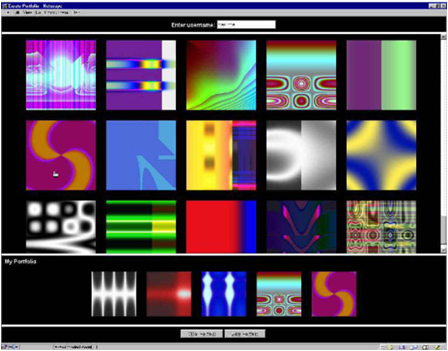
\includegraphics[width=8cm,bb=0 0 448 351]{figures/Dejavu.png}
  \caption{D\'{e}j\`{a} Vu}
  \label{fig:sample}
\end{figure}

\begin{figure}
  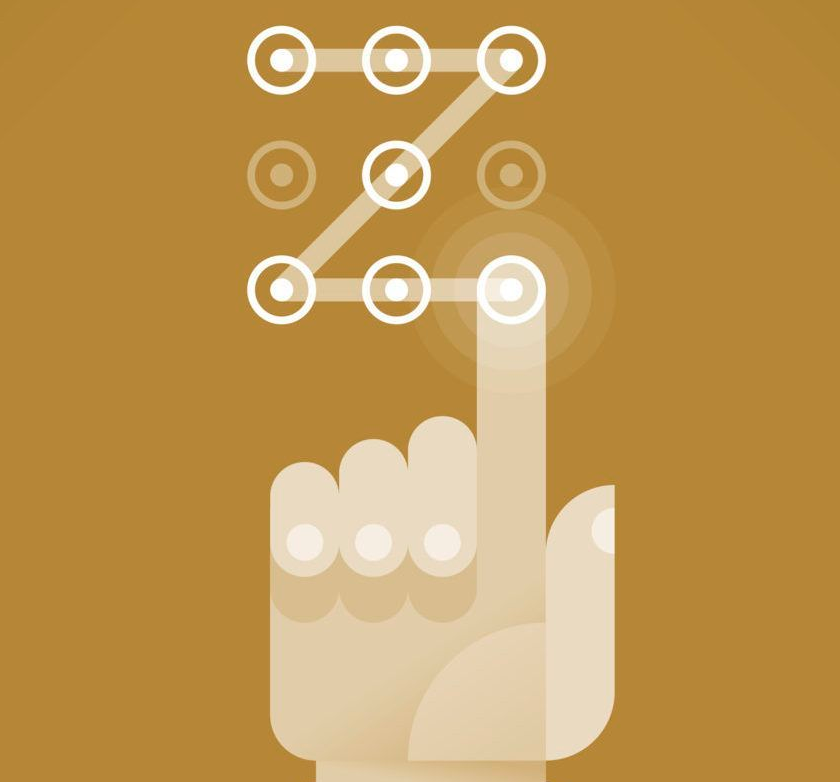
\includegraphics[width=8cm,bb=0 0 840 792]{figures/DAS.png}
  \caption{DAS Android}
  \label{fig:sample}
\end{figure}

We propose a new visual password generation system \textit{EpisoDAS},
with which users can generate strong password based on their
memory of visual patterns and episodic memories.
Users can either select answers based on the user's secret episodic memories or
draw a secret pattern represented by the pattern of selected answers.

Thus, users can recognize EpisoDas as a DAS system or
use it as an implementation of EpisoPass.


If the series of correct answers form a pattern
that is easy for the user to remember,
the user can select correct answers just like
using the DAS system.


\section{EpisoDAS}

% http://episopass.com/Amazon_john@example.com/Amazon123456

Figure \ref{EpisoDAS1} shows how a user can generate a password from
his episodic memories.

\begin{figure}
  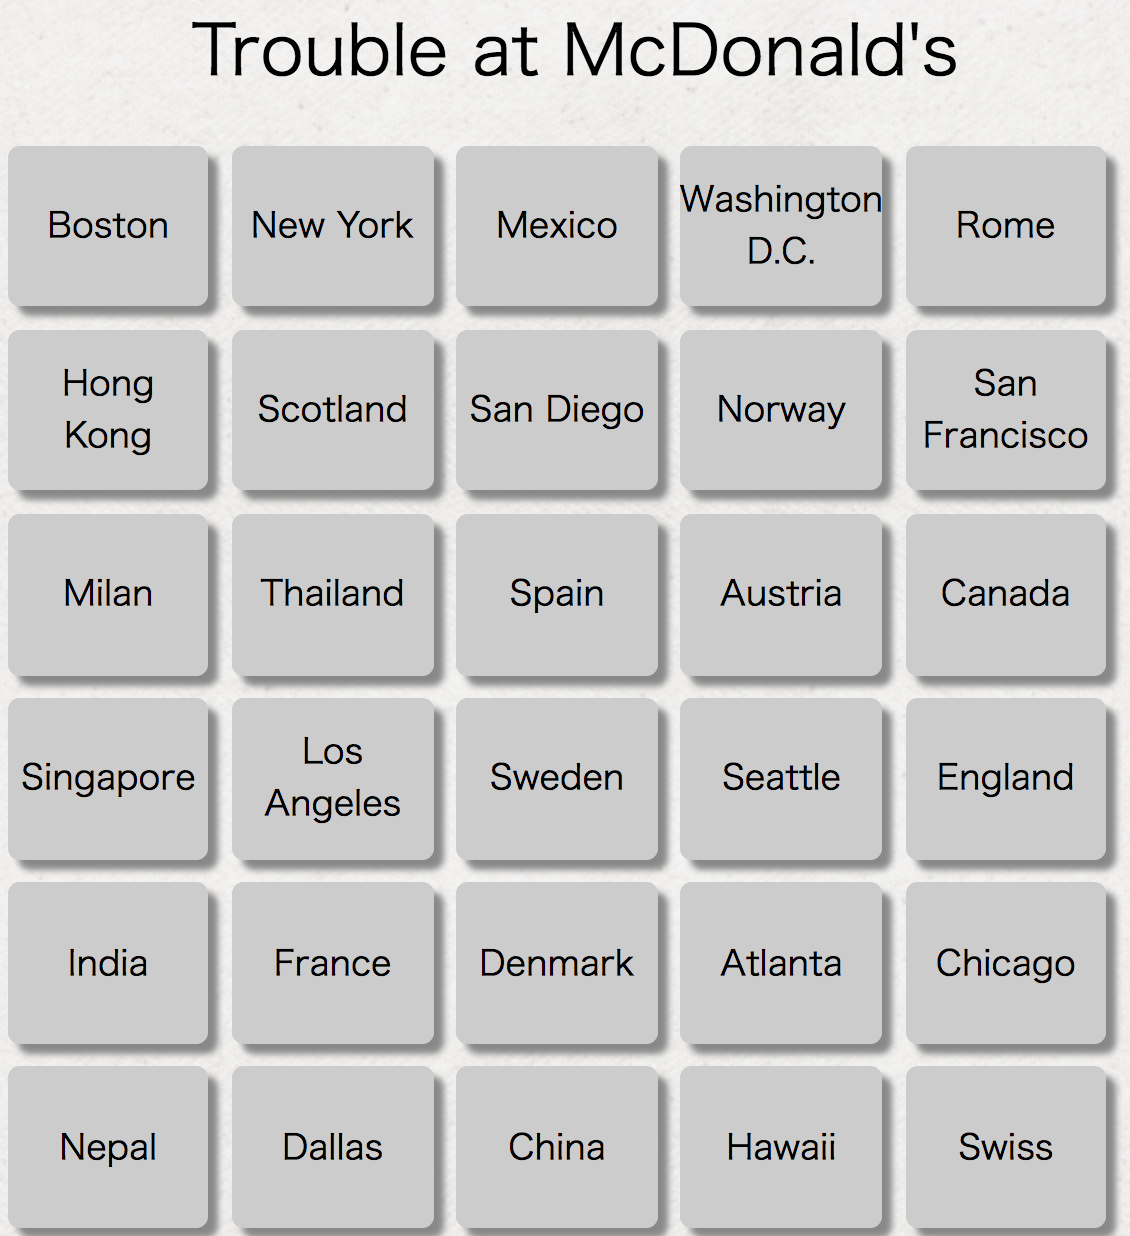
\includegraphics[width=9cm,bb=0 0 1130 1236]{figures/EpisoDAS1.png}
  \caption{First question}
  \label{EpisoDAS1}
\end{figure}

If the user remembers a trouble at MacDonald's in Boston,
he clicks ``Boston'', and the next question is displayed.
The same next question appears regardless of the selection
the user has made.

\begin{figure}
  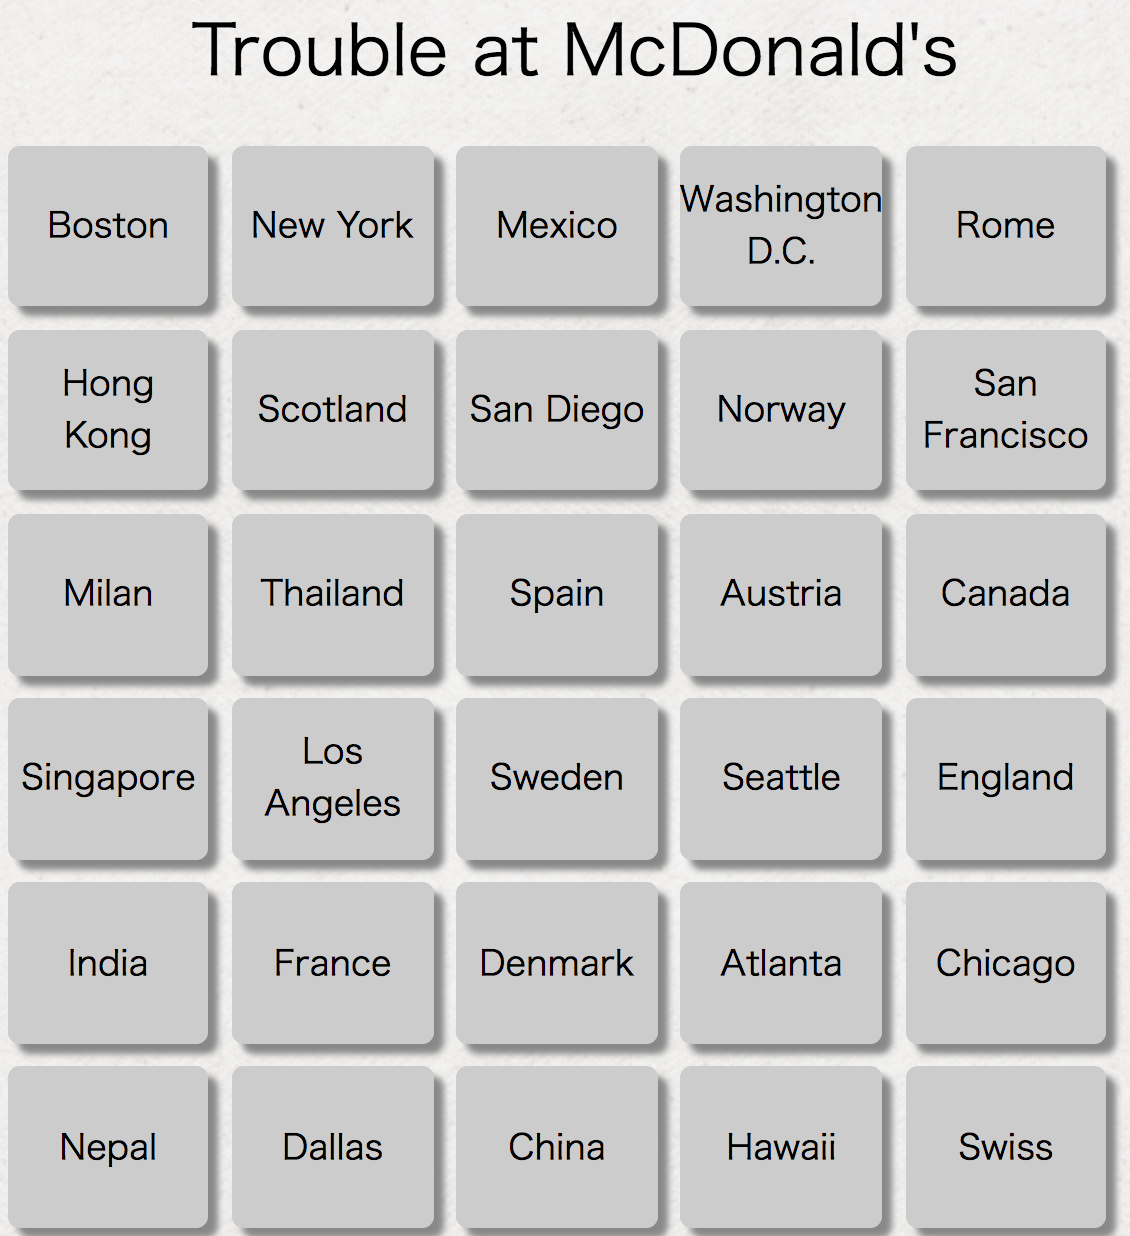
\includegraphics[width=9cm,bb=0 0 1130 1236]{figures/EpisoDAS1.png}
  \caption{Second question}
  \label{EpisoDAS2}
\end{figure}

If he remembers that he had a bad time at Los Angeles,
he clicks ``Los Angeles'', and another question is displayed.

After repeating the operation ten times,
the user can get his password.

\begin{figure}
  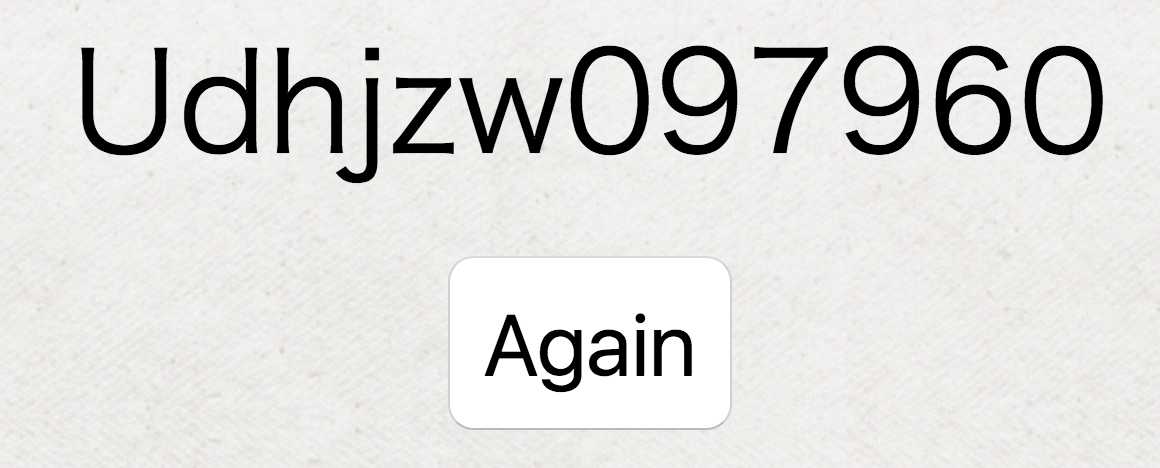
\includegraphics[width=9cm,bb=0 0 1160 468]{figures/result.png}
  \caption{Generated password}
  \label{EpisoDAS2}
\end{figure}

If the series of buttons are aligned next to each others,
the user can move the pointing device like below and get the password
without clicking buttons.

\begin{figure}
  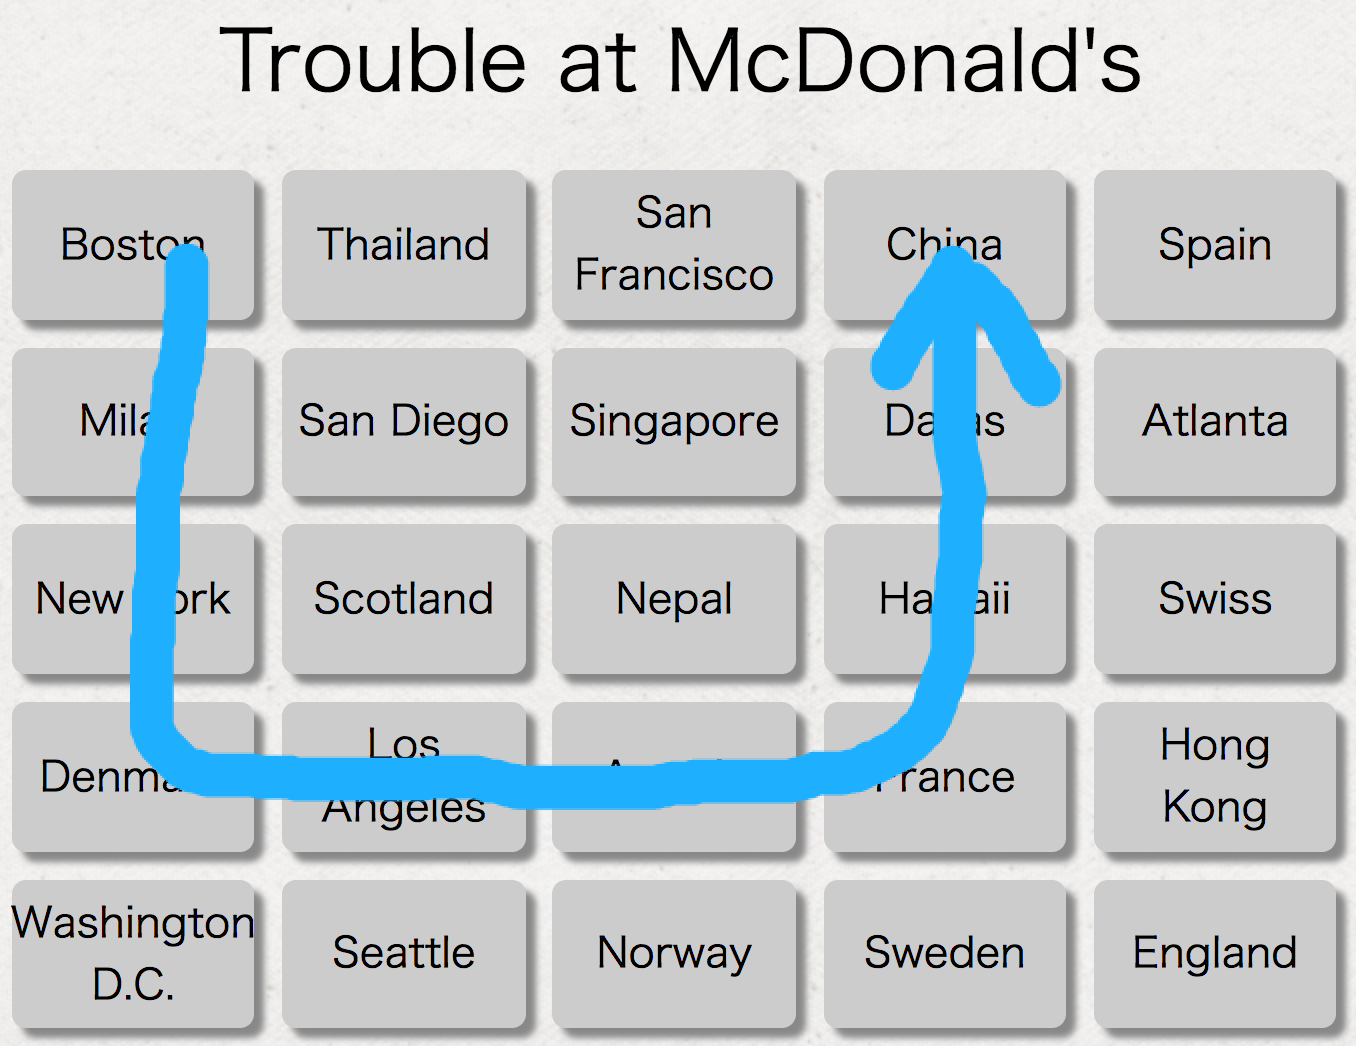
\includegraphics[width=9cm,bb=0 0 1130 1236]{figures/draw.png}
  \caption{Drawing a secret pattern}
  \label{EpisoDAS2}
\end{figure}

This operation is close to many conventional DAS systems.
Users can quickly retrieve his password just by
drawing a pattern on the EpisoDAS screen.

Using a conventional DAS system, users should be carefull about
remembering the DAS pattern.
DAS patterns may be more easily remembered than password texts,
but there is always some risks about forgetting them.
Using EpisoDAS, users can easily remember the DAS pattern
just by reading the questions and answers.
Users can be very sure that they will never forget the pattern,
because the pattern can be retrieved by answering the questions.

Figure xxxx shows how a user can use EpisoDAS on a login page,
using a browser extension software.
The extension shows a EpisoDAS window when a user tries to log into
an Web service, and after the user selects the right answers,
a password is generated from the input and pasted in to the
password text box.

\section{Registering a DAS pattern}

EpisoDAS is an extension to the EpisoPass system, and questions and
answers should be registered on the EpisoPass system.
After registering them, a user can register a DAS pattern
based on the question-answer pairs saved a

\section{Discussion}

* Saved as a single HTML file
* マスターパスワードが要らない
* 入力が高速 -
拡張機能を利用すると
記憶しているパスワード入力よりも高速なぐらいで入力できる

\section{Conclusion}

% \begin{acks}
% \end{acks}

% \bibliographystyle{ACM-Reference-Format}
\bibliography{sample-bibliography}

\end{document}
